\documentclass[11pt,a4paper]{article}
\usepackage[utf8]{inputenc}
\usepackage[T1]{fontenc}
\usepackage[french]{babel}
\usepackage{lmodern}
\usepackage{microtype}
\usepackage[margin=2cm,top=1.45cm,bottom=1.4cm]{geometry}
\usepackage[table]{xcolor}
\usepackage{graphicx}
\usepackage{needspace}
\usepackage{booktabs}
\usepackage{tabularx}
\usepackage{enumitem}
\usepackage[most]{tcolorbox}
\usepackage{titlesec}
\usepackage[hidelinks]{hyperref}
\newcommand{\numeroprojet}{5}
\newcommand{\titreprojet}{Valeur client et fidélisation : mieux cibler les clients à risque}
\newcommand{\membres}{Chris Boupassaia, Bertrand De Vertreuil, Améziane Haouanoh, Léonie Schmit}
\newcommand{\groupe}{Groupe 5}
\definecolor{principal}{HTML}{202020}
\definecolor{fondencadre}{HTML}{F4F4F4}
\setlength{\parindent}{0pt}
\setlength{\parskip}{0.22em}
\setlist{nosep,leftmargin=1.3em,topsep=2pt}
\titleformat{\section}{\large\bfseries\color{black}}{}{0em}{}
\titlespacing*{\section}{0pt}{0.45em}{0.12em}
\pagestyle{plain}
\newtcolorbox{enbref}{enhanced,colback=fondencadre,colframe=principal,boxrule=0pt,leftrule=4pt,arc=2pt,left=8pt,right=8pt,top=4pt,bottom=5pt,title={En bref},fonttitle=\bfseries,coltitle=principal,colbacktitle=fondencadre,toptitle=3pt,bottomtitle=0pt}
\AtEndDocument{\ifnum\value{page}>2 \par\vfill\begin{center}\color{red}\bfseries Attention : le résumé exécutif dépasse 2 pages.\end{center}\fi}
\begin{document}
\noindent{\small\color{black!65}Data Science sous R — ESME, Ingé3 2026-2027\hfill Projet n\textsuperscript{o}\,\numeroprojet{} — \groupe}\par
\vspace{0.4em}
{\Large\bfseries\color{black}Valeur client et fidélisation\par}
\vspace{0.12em}
{\large\bfseries\color{black}Mieux cibler les clients à risque\par}
\vspace{0.25em}
{\small \membres{}\hfill 8 novembre 2026\par}
\vspace{0.25em}\noindent\rule{\linewidth}{0.4pt}

\begin{enbref}
\begin{itemize}
\item \textbf{Un enjeu réel de fidélisation :} parmi les 1\,539 clients ayant acheté de janvier à septembre 2025, 26,8\,\% n'ont pas commandé au dernier trimestre.
\item \textbf{Un ciblage plus précis :} notre meilleur modèle distingue assez bien les clients à risque (score AUC de 0,838 sur le jeu de test).
\item \textbf{Une priorité :} contacter d'abord les clients à forte valeur et à risque élevé ; 49\,\% d'entre eux n'ont pas racheté, contre 8\,\% des clients à forte valeur et à risque faible dans le jeu de test.
\end{itemize}
\end{enbref}

\section{Le contexte et la question}
La boutique en ligne vend des produits dont les marges varient fortement selon les catégories. Envoyer la même promotion à tous les clients peut coûter cher, sans aider à retenir les plus intéressants. Nous avons cherché à savoir si leurs achats de janvier à septembre 2025 permettaient de repérer ceux qui ne commanderaient plus entre octobre et décembre. Le but est d'aider le marketing à choisir qui relancer en priorité.

\section{Ce que nous avons fait}
\begin{itemize}
\item \textbf{Données :} historique d'achats et profils de clients d'une boutique fictive, avec des données simulées sur l'année 2025 ; 1\,539 clients ont commandé pendant la période étudiée.
\item \textbf{Démarche :} nous avons comparé les habitudes d'achat, estimé le risque de non-réachat, puis croisé ce risque avec la marge apportée par chaque client. Nous avons également étudié les résultats de deux versions d'un e-mail commercial.
\item \textbf{Vérification :} les performances ont été mesurées sur des clients non utilisés pour construire les modèles. Nous avons aussi testé la stabilité des résultats.
\end{itemize}

\section{Les principaux résultats}
\begin{enumerate}
\item \textbf{Le risque peut être anticipé.} Le modèle retenu obtient un score de 0,838 sur 1 pour distinguer les clients qui rachètent de ceux qui ne rachètent pas. D'autres découpages donnent des scores autour de 0,80 : il faut donc rester prudent.
\item \textbf{Un seuil de 30\,\% permet de repérer davantage de départs.} À ce seuil, le modèle repère 75\,\% des clients sans nouvel achat et identifie correctement 76\,\% des clients qui rachètent.
\item \textbf{La valeur client aide à fixer la priorité.} Sur le jeu de test, 35 clients cumulent forte marge historique et risque élevé. Dans ce groupe, 49\,\% n'ont pas racheté, contre 8\,\% parmi les clients à forte valeur et à faible risque.
\end{enumerate}

\begin{figure}[ht]
\centering
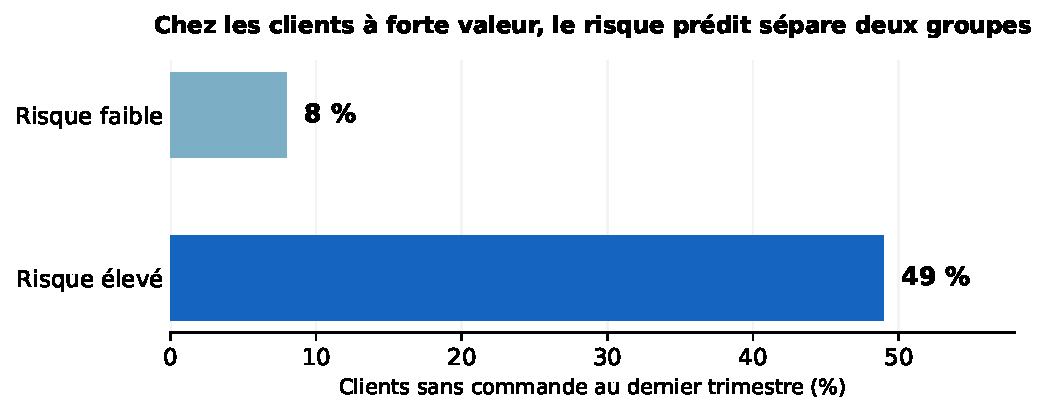
\includegraphics[width=0.90\linewidth]{figures/figure-cle.pdf}
\caption{Part de clients sans nouvel achat dans le jeu de test, parmi les clients à forte valeur.}
\end{figure}

\section{Nos recommandations}
\begin{center}
\rowcolors{2}{fondencadre}{white}
\begin{tabularx}{\linewidth}{>{\raggedright\arraybackslash}X >{\raggedright\arraybackslash}p{4.1cm} >{\centering\arraybackslash}p{1.5cm}}
\toprule
\textbf{Action} & \textbf{Effet recherché} & \textbf{Priorité}\\
\midrule
Relancer les clients à forte valeur dont le risque estimé dépasse 30\,\%. & Concentrer les offres sur les clients dont le départ serait le plus coûteux. & Haute\\
Personnaliser les messages selon les achats passés, sans remise systématique. & Encourager le réachat tout en préservant la marge. & Haute\\
Tester la campagne sur un petit groupe, avec un groupe témoin. & Mesurer les achats réellement gagnés et le coût des offres. & Haute\\
\bottomrule
\end{tabularx}
\end{center}

\Needspace{5\baselineskip}
\textbf{Concernant les e-mails :} la version B obtient davantage d'ouvertures (différence significative), mais l'écart sur les achats n'est pas concluant : seulement 20 achats ont été observés au total. Il serait donc prématuré d'affirmer qu'elle augmente les ventes.

\section{Limites et prochaines étapes}
\begin{itemize}
\item \textbf{Limites :} les données sont simulées et portent sur une seule année. Trois mois sans achat ne signifient pas forcément la perte définitive d'un client. Les marges sont estimées, notamment pour les ventes avec promotion, et le modèle peut se tromper. Les résultats observés ne prouvent pas qu'une relance sera efficace.
\item \textbf{Suite proposée :} utiliser plusieurs années d'achats, améliorer le calcul des marges et lancer un test de fidélisation avec groupe témoin. Suivre les taux de réachat, la marge supplémentaire et le coût des offres avant toute généralisation.
\end{itemize}

\end{document}
